% This is samplepaper.tex, a sample chapter demonstrating the
% LLNCS macro package for Springer Computer Science proceedings;
% Version 2.20 of 2017/10/04
%
\documentclass[runningheads, orivec]{llncs}

\usepackage[dvipdfmx]{graphicx}
\usepackage{tikz-cd}
\usepackage{mdframed}
\usepackage{amsmath, amssymb}
\makeatletter
\DeclareFontEncoding{LS2}{}{\@noaccents}
\makeatother
\DeclareFontSubstitution{LS2}{stix}{m}{n}

\DeclareSymbolFont{largesymbolsstix}{LS2}{stixex}{m}{n}

\DeclareMathDelimiter{\lbrbrak}{\mathopen}{largesymbolsstix}{"EE}{largesymbolsstix}{"14}
\DeclareMathDelimiter{\rbrbrak}{\mathclose}{largesymbolsstix}{"EF}{largesymbolsstix}{"15}
\newcommand{\newbrak}[2]{\genfrac{\lbrbrak}{\rbrbrak}{0pt}{}{#1}{#2}}


%\let\Bbbk\relax
%\usepackage[T1]{fontenc}
%\usepackage[straightbraces, mtphbi]{mtpro2}
%\usepackage{textcomp}
%\renewcommand{\rmdefault}{ptm}
%\usepackage[scaled=0.92]{helvet}

\usepackage{stmaryrd}
% Used for displaying a sample figure. If possible, figure files should
% be included in EPS format.
%
% If you use the hyperref package, please uncomment the following line
% to display URLs in blue roman font according to Springer's eBook style:
% \renewcommand\UrlFont{\color{blue}\rmfamily}


\begin{document}
%
\title{Advanced program calculation using typeclass in Coq}
%
%\titlerunning{Abbreviated paper title}
% If the paper title is too long for the running head, you can set
% an abbreviated paper title here
%
\author{Kosuke Murata\inst{1} \and
Emoto Kento\inst{1}}
%
\authorrunning{M. Kosuke and K. Emoto}
% First names are abbreviated in the running head.
% If there are more than two authors, 'et al.' is used.
%
\institute{Kyushu Institute of Technology, Japan\\
\email{murata@pl.ai.kyutech.ac.jp, emoto@ai.kyutech.ac.jp}}
%
\maketitle              % typeset the header of the contribution
%
\begin{abstract}
Program calculation, which is a programming technique to derive efficient but elusive programme from accessible but inefficient programme, is an important activity for developing program optimization. 

\keywords{Program calculation \and Functional programming \and Coq \and Interactive theorem proving.}
\end{abstract}
%
%
%
\section{Introduction}

Simple programme tend to be easy to implement, but inefficient and useless. On the contrary, efficient programme are useful but they require difficult programming techniques for implementation. Making ``program efficiency'' and ``easiness of implementation'' compatible is important challenge for study of programming. 

Program calculation~\cite{Bird:1988,Bird:1997} is programming technique to derive highly technical and efficient programme from simple and inefficient programme by using rules for programme. Of course, preserving semantics of programme is essential for correctness of program calculations. In this paper, correctness of program calculation means preserving semantics of programme. 

For certificating correctness of program calculation, Tesson, et al.~\cite{Tesson:2010} designed a tactic library for program calculation in Coq~\cite{}, which is an interactive theorem prover. Their tactic library has provided tactic notations for write Coq scripts like chains of equality, which is common in program calculation. They also formalized theory of lists~\cite{Bird:1988}, which provides a calculation rules for list-function base on Bird-Meertence Formalism (BMF). 

However, not only the list but also several algebraic datatypes (ADTs) such as natural numbers, binary trees and more general trees are essential for functional programming in practice. Fortunately, several studies describe calculation rules for arbitrary ADTs\cite{}. In this paper, we call such rules ``ADT-generic rules.'' ADT-generic rules are stated by using \( F \)-initial algebra and \( F \)-terminal coalgebra for modeling algebraic datatypes, and \emph{recursion schemes} such as catamorphism, anamorphism and paramorphism for modeling programs which can be recursively defined on arbitrary ADTs. 

The present paper aims to formalize ADT-generic rules described in Uustalu's paper~\cite{Uustalu:99}, which describes basic ADT-generic rules for basic recursion schemes such as catamorphism and anamorphism, and for little advanced recursion schemes such as futumorphism and histmorphism. 

In this study, we emphasize on using shallow embedding as much as possible. For proving theorems about programs by using interactive theorem provers, here are two styles to define semantics of domain languages: shallow embedding and deep embedding. The former is using the semantics of a host language as it as the semantics of a domain language, the latter is to construct another semantics of domain language on a host language. Deep embedding is flexible and has high power of expressions, but it tends to need high-cost proof. Unfortunately, depending on the way of constructing a semantics in the host language, it is difficult to get a ``runnable'' program. On the other hands, shallow embedding is less flexible, but the cost of proof tends to be low. Moreover, it is possible to make proof using a program that can be processed by a host language processing system, that is, it is actually runnable. From the perspective of program calculation in Coq, shallow embedding that uses Gallina, which is a core functional language in Coq, as a domain language makes it possible to safely derivation of runnable Gallina programs.

The organization of this paper is as follows. 後で書く.

\section{Preliminaries}\label{sec2}

In this section, we introduce Coq and its tactic library for program calculation proposed by Tesson, et al.~\cite{Tesson:2010}. We also introduce notions in basic category theory for describing ADT-generic theorems. 

\subsection{Overview of Coq and an tactic library for program calculation}

Coq~\cite{} is a popular interactive theorem prover. It based on the calculus of inductive constructions, which is a higher-order typed lambda calculus. It is widely used in computer science field, e.g. program verifications. A Coq script consists of definitions for data types, formula of propositions which we want to prove, and their proofs, and more. Coq proof are written using tactics, which are commands for construct proofs. Coq system has a sub-language Ltac for programming original tactics. Ltac provides \textbf{Tactic Notations} commands, which enable us to use various novel notations in Coq. For the details, see Coq reference manual \cite{}.

Tesson, et al.~\cite{Tesson:2010} designed and implemented a tactic library for program calculation in Coq using Ltac. Their tactic library has provided tactic notations which make it possible to write Coq script like equational reasoning, which is common notation in program calculation. In consideration of maintainability, we re-implemented our own tactic library using the same methods as theirs. 

The our library mainly for equational reasoning provides the following three tactics:
\begin{description}
\item{\underline{Tactic 1}.} \verb~Left = ~\( \langle\mathit{term}\rangle \)\verb~ {~ \( \langle\mathit{tactic}\rangle \) \verb~}~
\item{\underline{Tactic 2}.} \verb~= ~\( \langle\mathit{term}\rangle \)\verb~ {~ \( \langle\mathit{tactic}\rangle \) \verb~}~
\item{\underline{Tactic 3}.} \verb~= Right~
\end{description}
Fig. \ref{fig:Progress_of_interactive_proof} shows the Coq script using our library, for a proof of
\[
\forall ~ (x ~ y ~ z : \verb~nat~), ~ x = y \to z = x + x \to x + y = z, 
\]
and progress of its interactive proof in Coq IDE. For a goal \( t = s \), tactic 1 starts the proof by rewriting LHS \( t \) to the given \( \mathit{term} \) by using the specified tactic \( \mathit{tactic} \), to produce the next goal \( \mathit{term} = y \). This can be seen in the first step in Fig. \ref{fig:Progress_of_interactive_proof}, althought its specified \( \mathit{term} \) is exactly the same as the LHS of the goal and thus the goal is unchanged. Tactic 2 advance the chain in the similar way; see the 2nd through 4th steps in Fig. \ref{fig:Progress_of_interactive_proof}. Tactic 3 finished the chain. It directly proofs the current goal \( s = s \) by using \textbf{reflexivity}. Note that there term ``\( \verb~d := direction Rightwards~ : \mathsf{Prop}\)'' appearing in the Fig. \ref{fig:Progress_of_interactive_proof} is used to memorize the direction of the chain growth. 

To make script more shord and more readable, we implement short hands of these tactics. For instance, 
\begin{itemize}
\item{\underline{Tactic \( 2' \)}.} \verb~= ~\( \langle\mathit{term}\rangle \)
\end{itemize}
which is equal to \verb~= ~\( \langle \mathit{term} \)\verb~ { easy }~, and
\begin{itemize}
\item{\underline{Tactic \( 2'' \)}.} \verb~= ~\( \langle\mathit{term}\rangle \)\verb~ { by ~\( \langle\mathit{term}\rangle \) \verb~}~
\end{itemize}
which is equal to \verb~= ~\( \langle \mathit{term} \rangle \)\verb~ { rewrite ~\( \langle \mathit{term} \rangle \)\verb~ + rewrite <- ~\( \langle \mathit{term} \rangle \)\verb~ }~. 

\begin{figure}[t]
\centering
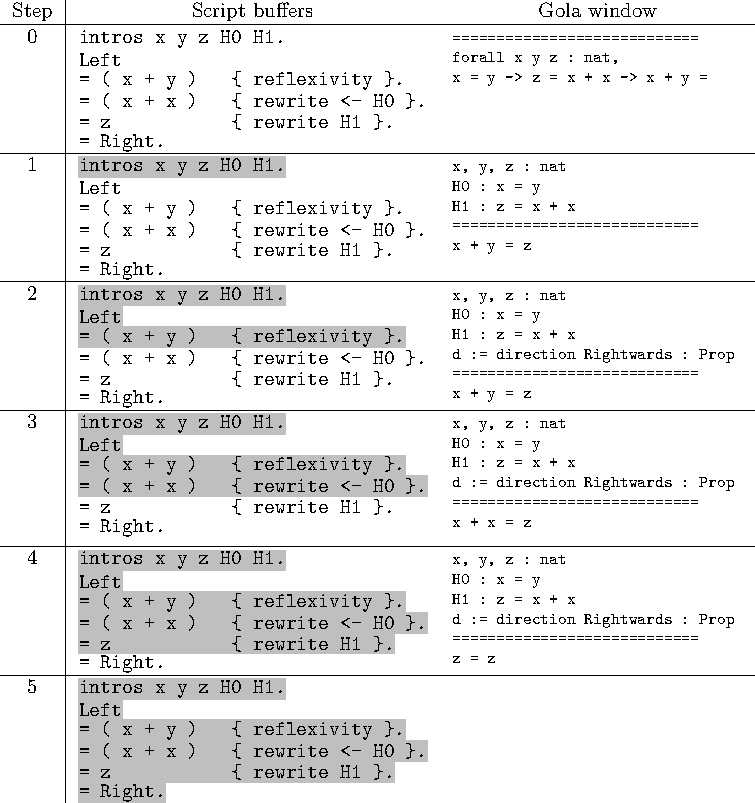
\includegraphics[width=0.7\linewidth]{figure2.pdf}

\caption{Progress of interactive proof on Coq IDE}
\label{fig:Progress_of_interactive_proof}
\end{figure}
In this paper, in order to improve readability, we write Coq scripts using roman and san serif fonts such as mathematical expressions, instead of typewriter fonts. 

\subsection{Basic notions of category theory}

We use basic notions of category theory for describing ADT-generic theorems. We work on the category \( \mathbf{Set} \), which is category of set and functions.

Given two sets \( A \), \( B \), we write \( A * B \) for product (just like \verb~Coq.Init.Datatypes~, the Coq standard library), and \( A + B \) for sum. We write \( \verb~fst~ : A * B \to A \) and \( \verb~snd~ : A * B \to B \) for the left and right projection function, \( \verb~inl~ : A \to A + B \) and \( \verb~inr~ : B \to A + B \) for the constructors for sum. 

We use also following notations, which are non-standard in Coq but familiar in program calculation, just like \cite{Uustalu:99}. For \( f : A \to B \) and \( g : A \to C \), we use \( \langle f, g \rangle : A \to B * C \) for unique morphism \( h \) such that \( \verb~fst~ \circ h = f \) and \( \verb~snd~ \circ h = g \). For \( f : A \to C \) and \( g : B \to C \), we use \( [f, g] : A + B \to C \) for unique morphism \( h \) such that \( h \circ \verb~inl~ = f \) and \( h \circ \verb~inr~ = g \). Fig. \ref{fig:def_product_sum_morphisms}. shows the definitions for such morphisms in Coq. 

\begin{figure}[t]
\[
\begin{array}{l}
\mathbf{Definition}~\verb~fprod~~\{A~B~C : \mathsf{Type}\}~(f : A \to B)~(g : A \to C) : A \to B * C := \\
~~\lambda~(x : A) \Rightarrow (f~x, g~x).\\
\mathbf{Definition}~\verb~fsum~~\{A~B~C : \mathsf{Type}\}~(f : A \to B)~(g : A \to C) : A + B \to C := \\
~~\lambda ~ (x : A + B) \Rightarrow \begin{array}[t]{l}
\mathbf{match}~x~\mathbf{with}\\
| ~ \verb~inl~~x \Rightarrow f~x \\
| ~ \verb~inr~~x \Rightarrow g~x \\
\mathbf{end}.
\end{array}\\
\mathbf{Notation}~\verb~"~ \langle f,g \rangle\verb~"~ := (\verb~fprod~~f~g).\\
\mathbf{Notation}~\verb~"~ [ f,g ]\verb~"~ := (\verb~fsum~~f~g).
\end{array}
\]

\caption{The definitions for product and sum of morphisms in Coq}
\label{fig:def_product_sum_morphisms}
\end{figure}

\begin{figure}[t]
\[
\begin{array}{lllclll}
\verb~fst~ \circ \langle f, g \rangle &=& f &\quad& {} [f, g] \circ \verb~inl~ &=& f \\
\verb~snd~ \circ \langle f, g \rangle &=& g && {} [f, g] \circ \verb~inr~ &=& g \\
\langle \verb~fst~, \verb~snd~ \rangle &=& \mathit{id} && [\verb~inl~, \verb~inr~] &=& \mathit{id}
\end{array}
\]

\caption{Rules for product and coproduct}
\end{figure}

We use traditional way for modeling datatypes, which use \( F \)-initial algebras and terminal coalgebras where \( F : \mathbf{Set} \to \mathbf{Set} \) is a polynomial functor. For a polynomial functor \( F : \mathbf{Set} \to \mathbf{Set} \), we write \( ( \mu F , \mathsf{in}_F ) \) for the \( F \)-initial algebra, \( (\nu F , \mathsf{out}_F ) \) for the \( F \)-terminal coalgebra. Note that for any polynomial functor \( F : \mathbf{Set} \to \mathbf{Set} \), there exists unique a \( F \)-initial algebra and a \( F \)-terminal coalgebra up to isomorphism. We also use polynomial functors indexed by constant set \( A \); e.g. \( F_A : \mathbf{Set} \to \mathbf{Set} \) such that \( F_A(X) = \mathbf{1} + A * X \). From the aspect of formilization, indexed functors just like \( F_A(X) \) can be assumed that is partial application of bifunctor \( F : \mathbf{Set} \to \mathbf{Set} \to \mathbf{Set} \).

Let \( F \colon \mathbf{Set} \to \mathbf{Set} \) be a polynomial functor, and \( (\mu F, \mathsf{in}_F) \) be an initial \( F \)-algebra. Given a morphism \( \varphi \colon F\,X \to X \), the morphism \( \llparenthesis \varphi \rrparenthesis \colon F\,\mu F \to \mu F \) is \emph{catamorphism}\footnote{The term `catamorphism' is derived from the greek preposition \(\mathit{\kappa\alpha\tau\alpha}\) meaning `downwards'.} if following diagram commutes:
\[
\begin{tikzcd}
F\,\mu F \ar[d, "{F\;\llparenthesis \varphi \rrparenthesis}"']\ar[r, "{\mathsf{in}_F}"] & \mu F \ar[d, "{\llparenthesis \varphi \rrparenthesis}"] \\
F\,X \ar[r, "{\varphi}"'] & X
\end{tikzcd}.
\]
In other words, \( \llparenthesis f \rrparenthesis \) is characterized by the universal property:
\[
f \circ \mathsf{in}_F = \varphi \circ F\,f \iff f = \llparenthesis \varphi \rrparenthesis .
\]
Anamorphism とかについても後で書く.


\section{Modeling Datatypes in Coq}

In this section, we propose a way to models concepts to model datatypes in Coq. Types and functions in Coq can be regarded as object and morphisms in category \( \mathbf{Set} \). 

\begin{figure}[tbhp]
\[
\begin{array}{l}
\mathbf{Inductive}~\verb~PolyF~ : \mathsf{Type} := \\
\begin{array}{llll}
| & \verb~zer~ &:& \verb~PolyF~ \\
| & \verb~one~ &:& \verb~PolyF~ \\
| & \verb~arg1~ &:& \verb~PolyF~ \\
| & \verb~arg2~ &:& \verb~PolyF~ \\
| & \verb~Sum~ &:& \verb~PolyF~ \to \verb~PolyF~ \to \verb~PolyF~ \\
| & \verb~Prod~ &:& \verb~PolyF~ \to \verb~PolyF~ \to \verb~PolyF~ .
\end{array}\\
\\
\mathbf{Inductive}~\verb~inst~~(F : \verb~PolyF~)~(A~X : \mathsf{Type}) : \mathsf{Type} := \\
~~ \mathbf{match}~F~\mathbf{with}\\
~~ \begin{array}{llll}
| & \verb~zer~ &\Rightarrow& \verb~Empty_set~ \\
| & \verb~one~ &\Rightarrow& \verb~Unit~ \\
| & \verb~arg1~ &\Rightarrow& A \\
| & \verb~arg2~ &\Rightarrow& X \\
| & \verb~Sum~~F~G &\Rightarrow& (\verb~inst~~F~A~X) + (\verb~inst~~G~A~X) \\
| & \verb~Prod~~F~G &\Rightarrow& (\verb~inst~~F~A~X) * (\verb~inst~~G~A~X)
\end{array}\\
~~\mathbf{end}.\\
\\
\mathbf{Notation}~\verb~"~ \llbracket F \rrbracket \verb~"~ := (\verb~inst~~F).\\
\\
\mathbf{Fixpoint}~\verb~fmap~~(F : \verb~PolyF~)~\{A_0~A_1~X_0~X_1 : \mathsf{Type}\}\\
\qquad (f : A_0 \to A_1)~ (g : X_0 \to X-1) : \llbracket F \rrbracket ~ A_0 ~ X_0 \to \llbracket F \rrbracket ~ A_1 ~ X_1\\
\qquad := 
\begin{array}[t]{l}
\mathbf{match}~F~\mathbf{with} \\
\begin{array}[t]{llll}
\mid & \verb~zer~ &\Rightarrow& \mathrm{id} \\
\mid & \verb~one~ &\Rightarrow& \mathrm{id} \\
\mid & \verb~arg1~ &\Rightarrow& f \\
\mid & \verb~arg2~ &\Rightarrow& g \\
\mid & \verb~Sum~~F~G &\Rightarrow& \lambda x \Rightarrow 
\begin{array}[t]{l}
\mathbf{match}~x~\mathbf{with}\\
\begin{array}{lll}
\verb~inl~~x &\Rightarrow& \verb~inl~~(\verb~fmap~~F~f~g~x) \\
\verb~inr~~x &\Rightarrow& \verb~inr~~(\verb~fmap~~F~f~g~x) \\
\mathbf{end}
\end{array}
\end{array}\\
\mid & \verb~Prod~~F~G &\Rightarrow& \lambda x \Rightarrow (\verb~fmap~~f~g~(\verb~fst~~x), \verb~fmap~~G~f~g~x~(\verb~snd~~x)) 
\end{array}\\
\mathbf{end}.
\end{array}\\
\\
\mathbf{Notation}~\verb~"~ F [ f ] \verb~"~ := (\verb~@fmap~~F~\_~\_~\_~\_~\mathrm{id}~f)~ (\text{at level 10}).
\end{array}
\]

\caption{The definitions for polynomial functor in Coq}
\label{fig:def_of_initial_alg}
\end{figure}

\subsection{Polynomial Functor}

Fig. \ref{fig:def_of_initial_alg}. shows the definitions for polynomial functor in Coq. Functor consists of following two mappings: mappings from object to object, and mappings from morphisms to morphisms. To define polynomial functor inductively, we first define \( \verb~PolyF~ \), which is the type for AST (Abstract Syntax Tree) of polynomial functor, and then use it to define following two mappings: 
\begin{itemize}
\item \( \llbracket F \rrbracket : \mathsf{Type} \to \mathsf{Type} \to \mathsf{Type}\)  (\( \verb~inst~~F \)) is to map from types to types. 
\item \( F\lbrbrak {-} \rbrbrak [{-}] \colon (A_0 \to A_1) \to (X_0 \to X_1) \to \llbracket F \rrbracket ~ A_0 ~ X_0 \to \llbracket F \rrbracket ~ A_1 ~ X_1 \)(\verb~fmap~) is mapping from morphisms to morphisms.
\end{itemize}
These definitions are for bifunctor, but we can get definitions for functor by partial applications, i.e. \( \llbracket F \rrbracket ~ A \) and \( F[@\mathrm{id}~A]({-}) \) define a functor (indexing by type \( A \)). 

Polynomial functors must satisfy the functor laws, so we proved following 2 lemmas for functor laws by using easy induction on \( F \). 
\begin{itemize}
\item 
\(\begin{array}[t]{l}
\mathbf{Lemma}~ \verb~fmap_functor_distr~ : \\
\quad \forall ~ (F : \verb~PolyF~) ~ \{ A ~ X_0 ~ X_1 ~ X_2 : \mathsf{Type} \} ~ (g_0 : X_0 \to X_1) ~ (g_1 : X_1 \to X_2), \\
\qquad F \lbrbrak @ \mathrm{id}~A \rbrbrak [g_1 \circ g_0] = F [g_1] \circ F [g_0]
\end{array}
\)

\item \(\begin{array}[t]{l}
\mathbf{Lemma}~ \verb~fmap_functor_id~ : \\
\quad \forall ~ (F : \verb~PolyF~) ~ \{ A ~ X : \mathsf{Type} \} ~ (g_0 : X_0 \to X_1) ~ (g_1 : X_1 \to X_2), \\
\qquad F \lbrbrak @ \mathrm{id}~A \rbrbrak [\verb~@~\mathrm{id}~X] = \mathrm{id}
\end{array}
\)
\end{itemize}

Next, we define \( F \)-initial algebras using type class. Fig. \ref{fig:f_initial_alg}. shows the definitions for \( F \)-initial algebras using type class in Coq.

\begin{figure}[t]
\[
\begin{array}{l}
\mathbf{Class}~\begin{array}[t]{l}
\verb~F_initial_algebra~~(F : \verb~PolyF~)~(A : \mathsf{Type})~(\mu F : \mathsf{Type}) \\
(c : \forall ~ (X : \mathsf{Type}), (\llbracket F \rrbracket ~ A ~ X \to X) \to ( \mu F \to X) ) := 
\end{array} \\
~~\{\\
~~~~\begin{array}{lll}
\verb~cata~ := c; \\
\verb~in_~ &:& \llbracket F \rrbracket ~ A ~ \mu F \to \mu F ; \\
\verb~cata_charn~ &:& \forall ~ (X : \mathsf{Type})~(f : \mu F \to X)~ (\varphi : \llbracket F \rrbracket ~ A ~ X \to X),\\
&&~~~~ f \circ \verb~in_~ = \varphi \circ F[f] \leftrightarrow f = \verb~cata~~X~\varphi
\end{array}\\
~~\}.\\
\\
\mathbf{Notation}~\verb~"~\llparenthesis f \rrparenthesis\verb~"~ := (\verb~cata~~\_~\_~f)~(\text{at level 5}).
\end{array}
\]

\caption{Definitions for \( F \)-initial algebras using type class in Coq}
\label{fig:f_initial_alg}
\end{figure}

Initial algebras and catamorphisms satisfy the following 3 properties, where
\[
\mathbf{Variable}~\begin{array}[t]{l}
(F : \verb~PolyF~) ~ (A : \mathsf{Type}) ~ ( \mu F : \mathsf{Type}) \\
(c : \forall ~ (X : \mathsf{Type}), ~ (\llbracket F \rrbracket ~ A ~ X \to X) \to (\mu F \to X) ) \\
(\mathit{ia} : \verb~F_initial_algebra~ ~ F ~ A ~ \mu F ~ c).
\end{array}
\]
\begin{itemize}
\item \(
\begin{array}[t]{l}
\mathbf{Proposition}~\verb~cata_cancel~ : \\
\qquad \forall ~ (X~Y : \mathsf{Type}) ~ (\varphi : \llbracket F \rrbracket ~ A ~ X \to X), \\
\qquad\qquad \llparenthesis \varphi \rrparenthesis \circ \verb~in_~ = \varphi \circ F[\llparenthesis \varphi \rrparenthesis].
\end{array}
\)

\item \(\mathbf{Proposition}~\verb~cata_refl~ : \llparenthesis \verb~in_~ \rrparenthesis = \mathrm{id}\)

\item \(
\begin{array}[t]{l}
\mathbf{Proposition}~\verb~cata_fusion~ : \\
\qquad \forall ~ (X~Y : \mathsf{Type}) ~ (\varphi : \llbracket F \rrbracket ~ A ~ X \to X) ~ (\psi : \llbracket F \rrbracket ~ A ~ Y \to Y) ~ (f : X \to Y ), \\
\qquad\qquad f \circ \varphi = \psi \circ F[f] \to f \circ \llparenthesis \varphi \rrparenthesis = \llparenthesis \psi \rrparenthesis.
\end{array}
\)
\end{itemize}
Fig. \ref{fig:proof_catamorphism} shows the Coq proof of \verb~cata_fusion~. 


\begin{figure}[t]
\[
\begin{array}{l}
\mathbf{Proposition}~\verb~cata_fusion~ : \\
\qquad \forall ~ (X~Y : \mathsf{Type}) ~ (\varphi : \llbracket F \rrbracket ~ A ~ X \to X) ~ (\psi : \llbracket F \rrbracket ~ A ~ Y \to Y) ~ (f : X \to Y ), \\
\qquad\qquad f \circ \varphi = \psi \circ F[f] \to f \circ \llparenthesis \varphi \rrparenthesis = \llparenthesis \psi \rrparenthesis.\\
\mathbf{Proof}.\\
\quad \begin{array}[t]{ll}
\verb~intros~; ~ \verb~apply~ ~\verb~cata_charn~. \\
\mathbf{Left} \\
= (f \circ ( \llparenthesis \varphi \rrparenthesis \circ \verb~in_~ )). \\
= ( f \circ \varphi \circ F[\llparenthesis \varphi \rrparenthesis ] ) & \{ \mathbf{by} ~ \verb~cata_cancel~ \}. \\
= ( \psi \circ (F[f] \circ F[\llparenthesis \varphi \rrparenthesis ])) & \{ \mathbf{by} ~ H \}. \\
= ( \psi \circ F[f \circ \llparenthesis \varphi \rrparenthesis ] ) & \{ \mathbf{by} ~ \verb~fmap_functor_distr~ \}. \\
= \mathbf{Right}.\\
\end{array}\\
\mathbf{Qed}.
\end{array}
\]

\caption{A coq proof for catamorphism fusion-law, using tactic libraries}
\label{fig:proof_catamorphism}
\end{figure}


\subsection{Instanciation of the Class for initial algebra}

As a benefit of using type class for definition for initial algebra, it is possible to use the theorems for runnable Coq programs. 

First, we give an example of making \verb~nat~ an instance of \verb~F_initial_algebra~, where \verb~nat~ is standard type of natural numbers in Coq. The catamorphism of nat can define as follows:
\[
\begin{array}{l}
\mathbf{Definition}~\verb~cata_nat~~(X : \mathsf{Type})~(f : \verb~unit~ + X \to X) : \verb~nat~ \to X :=\\
\qquad \mathbf{fix}~\verb~cataf~~(n : \verb~nat~) := \begin{array}[t]{l}
       \mathbf{match}~n~\mathbf{with}\\
       \begin{array}{llll}
       | & \verb~O~    &\Rightarrow& f ~ (\verb~inl~ ~ ()) \\
       | & \verb~S~ ~ n' &\Rightarrow& f ~ (\verb~inr~ ~ (\verb~cataf~ ~ n')) 
       \end{array}\\
       \mathbf{end}.
       \end{array}
\end{array}
\]
Now, we can define \verb~Nat_IA~, which is an instance of \verb~F_initial_algebra~, as follows.
\[
\begin{array}{l}
\mathbf{Instance}~\verb~Nat_IA~ : \\
\qquad \verb~F_initial_algebra~~(\verb~Sum~~\verb~one~~\verb~arg2~)~\verb~unit~~\verb~cata~~\verb~cata_nat~ :=\\
\qquad \{\\
\qquad \qquad \verb~in_~ := [\lambda ~ x \Rightarrow \verb~O~, ~ \verb~S~];\\
\qquad \}.\\
\end{array}
\]
There are incomplete proofs of \verb~cata_charn~, but the proof is easy to complete (see Appendix). \verb~Nat_IA~ make us possible to evaluate catamorphisms in \verb~nat~, therefore, if Coq system reads following command: 
\[
\mathbf{Eval}~\mathrm{cbv}~\mathrm{in}~ (\lambda (y : \verb~nat~) \Rightarrow \llparenthesis [ \lambda \_ \Rightarrow y, S ] \rrparenthesis) ~ 100 ~ 11.
\]
it will return the answer, 111.

\section{More advanced recursion schemes}




\section{Related Work}

Furthermore, some research\cite{} uses interactive theorem prover such as Coq and Agda. 

\section{Conclusion and Future Work}





%
% ---- Bibliography ----
%
% BibTeX users should specify bibliography style 'splncs04'.
% References will then be sorted and formatted in the correct style.
%
\bibliographystyle{splncs04}
\bibliography{bibliography}
%

\appendix
\section{Coq Proof for Instantiation of Nat}

{\small
\begin{verbatim}
Instance Nat_ia :
  F_initial_algebra (Sum one arg2) unit nat cata_nat :=
  {
    in_  := [ fun x => O , S ];
  }.
Proof.
  intros X f φ.
  split.
  - intros H. unfold cata_nat.
    extensionality x.
    induction x.
    + specialize (equal_f H (inl tt)) as H0; cbv in H0.
      exact H0.
    + specialize (equal_f H (inr x)) as H1; cbv in H1.
      rewrite <- IHx.
      exact H1.
  - intros H; extensionality x; induction x.
    + rewrite H. induction a. easy.
    + rewrite H; easy.
Qed.
\end{verbatim}
}

\end{document}
